\documentclass{article}
\usepackage[utf8]{inputenc}
\usepackage{amsmath,amsfonts,amssymb}
\usepackage{graphicx}
\usepackage{booktabs}
\usepackage{multicol}
\usepackage{lipsum}
\usepackage[a4paper, total={6in, 8in}]{geometry}

\newtheorem{theorem}{Model}[section]
\newtheorem{corollary}{Corollary}[theorem]
\newtheorem{proof}{Proof}[corollary]

\title{Analysis on Period vs. Angle, Period vs. Length \& Q Factor of Pendulum}
\author{Zixuan Fan (fanzixu2)}
\date{09/18/2023}

\begin{document}

\maketitle

\section{Introduction}
In this lab report, we analyse the how the angle at which a pendulum is released, as well as the length that the pendulum is released, correlates with the period of the pendulum. Additionally, by computing the Q Factor [2], we will analyse the damping effect on the pendulum's period as the angle decreases. Finally, we will assess the how the damping effect correlates with the pendulum's length by calculating the Q Factor at each length. For this lab report, we will assume the rod of our pendulum stand is rigid, massless, and perfectly orthogonal to the pendulum stand; and the string of our pendulum is massless, always stretched, and has negligible air resistance. Our experimental results indicate that the at an release angle of 1.57 $\pm$ 0.01rad, the pendulum's period decreases exponentially with their release angle, as induced by errors regarding friction of the string and air resistance of the pendulum. Moreover, the observed exponential decay of the pendulum's amplitude over time corresponds to a Q Factor of 200 $\pm$1 derived through fitting function to graph, which aligns with the Q Factor of 196 $\pm$ 5 derived from counting oscillation. Furthermore, at a release angle of 1.05 $\pm$ 0.01rad, the correlation between the pendulum's length and its period is evident, with longer lengths leading to increased periods. Finally, through calculating and plotting 5 Q factors (292,288,276,264,248 $\pm$ 1) against each length (10.0,15.0,20.0,25.0,30.0 $\pm$ 0.1cm), we deduced that the damping effect is more pronounced in longer pendulum lengths. \\

\noindent Utilizing an experimental set-up that minimizes asymmetry and maintains the motion of the pendulum in a single plane, we will gather data points regarding the period of pendulum with regards to both angle and length, as well as graphing and analysing these data points in data analysis. The equations we used in data analysis are listed below [2]: 
\begin{equation}
 \theta(t) = \theta_0 e^{-t/\tau} \cos(2\pi \frac{t}{T}+\phi_0)
\end{equation}
In equation \textbf{(1)}, $\theta$ is the angle of the pendulum in rad,  $\theta_0$ is the release angle of the pendulum in rad, $t$ is the time in seconds, $\tau$ is in seconds, $T$ is the maximum period (the period in the first cycle) of pendulum in seconds, and $\phi_0$ is a phase shift constant. 
\begin{equation}
 Q=\pi \frac{\tau}{T}=\pi
\end{equation}
In addition to the same terms in equation \textbf{(1)}, in equation \textbf{(2)}, $Q$ is the Q factor, a constant.
\begin{equation}
 \theta(t) = \theta_0 e^{-t/\tau} 
\end{equation}
Using to the same terms in equation \textbf{(1)}, equation \textbf{(3)} is a deviation of equation \textbf{(1)}

\section{Experimental Set-up}

The experimental set-up consists of suspending a golf ball from a horizontal wooden beam using double wool strings with adjustable length, as demonstrated in \textbf{Figure 1}.

\begin{figure}[!htb]
	\centering
	\includegraphics[scale=0.025, angle = 270]{experimental_setup_pendulum.jpg}
	\caption{Experimental Set-up of The Pendulum}
	\label{fig_angle}
\end{figure}

 The string of pendulum has a vertical length of 37.5 $\pm$ 0.1cm, and the golf ball along with the tape has a combined weight of 45.0 $\pm$ 0.1g. Wool strings were chosen as their masses are light enough to be ignored. Additionally, the video capture device has a frame rate of 30 frames per second.

\subsection{Improvements for The Set-up that Eliminate Asymmetry}


To maintain symmetry during experimentation, data was collected from both the negative (left) and positive (right) sides of the pendulum release. This approach minimizes errors stemming from the inherent asymmetry in the set-up. \\
\indent Efforts were also made to reduce this inherent asymmetry by adjusting the knot on the pendulum string to the lowest point on the wooden stand, thereby aligning the string with the symmetrical center line. \\
\indent Moreover, the golf ball is tied up using two strings to ensures that the motion of the ball stays in the same plane, which prevents asymmetry caused by circular motion of the ball, had the ball been hanged from only one string from the wooden beam.

\section{Data Analysis}

\subsection{Justification for Measurements of Uncertainty}

The most significant uncertainty within the experiment arises from the measurement of the angle, the length, and the period of the pendulum. Additionally, the friction between the string and the stand, and the influence of air resistance during pendulum swings could have contributed to an increased level of uncertainty. However, these two errors lead to a systematic shift in the data points. Unlike the random error in measurement, which causes fluctuations in individual data points, these systematic errors are far less prominent at increasing the uncertainty of individual data points. A further analysis of these two systematic errors will be provided in section 3.2.1.

The measurements for angles are done using an angle-meter with a step of $\pm$1 degree, equivalent to $\pm 1*\pi/180= \pm0.02$ in rad, as observable in \textbf{Figure 1}. Since the angle-meter is an analogue instrument, the uncertainty of Angle should be $\pm 0.02/2= \pm0.01$ rad.

 The measurements for periods and time are done using a digital tracker with a step of $ \frac{1.00 s}{30 frames}=0.03 s$ [1]. Since the tracker is a digital instrument, the uncertainty of period should be $\pm$ 0.03 second.
 
 The measurement for lengths of pendulum are done using a ruler with a step of $\pm$0.2 cm. Since the ruler is an analogue instrument, the uncertainty of lengths should be $\pm 0.2/2= \pm0.1$ cm.
 
 In future, all of these uncertainties caused by measurement can be reduced by selecting measuring instruments with smaller steps.


\subsection{Relationship between Angle and Period of Pendulum}

\subsubsection{Graphing and Analysing Figure 2}
The pendulum was released at 1.57 $\pm$ 0.01rad from both side of the stand. Importing gathered data into a provided python program, we were able to graph the period of pendulum against angles in \textbf{Figure 2}:

\begin{figure}[!htb]
	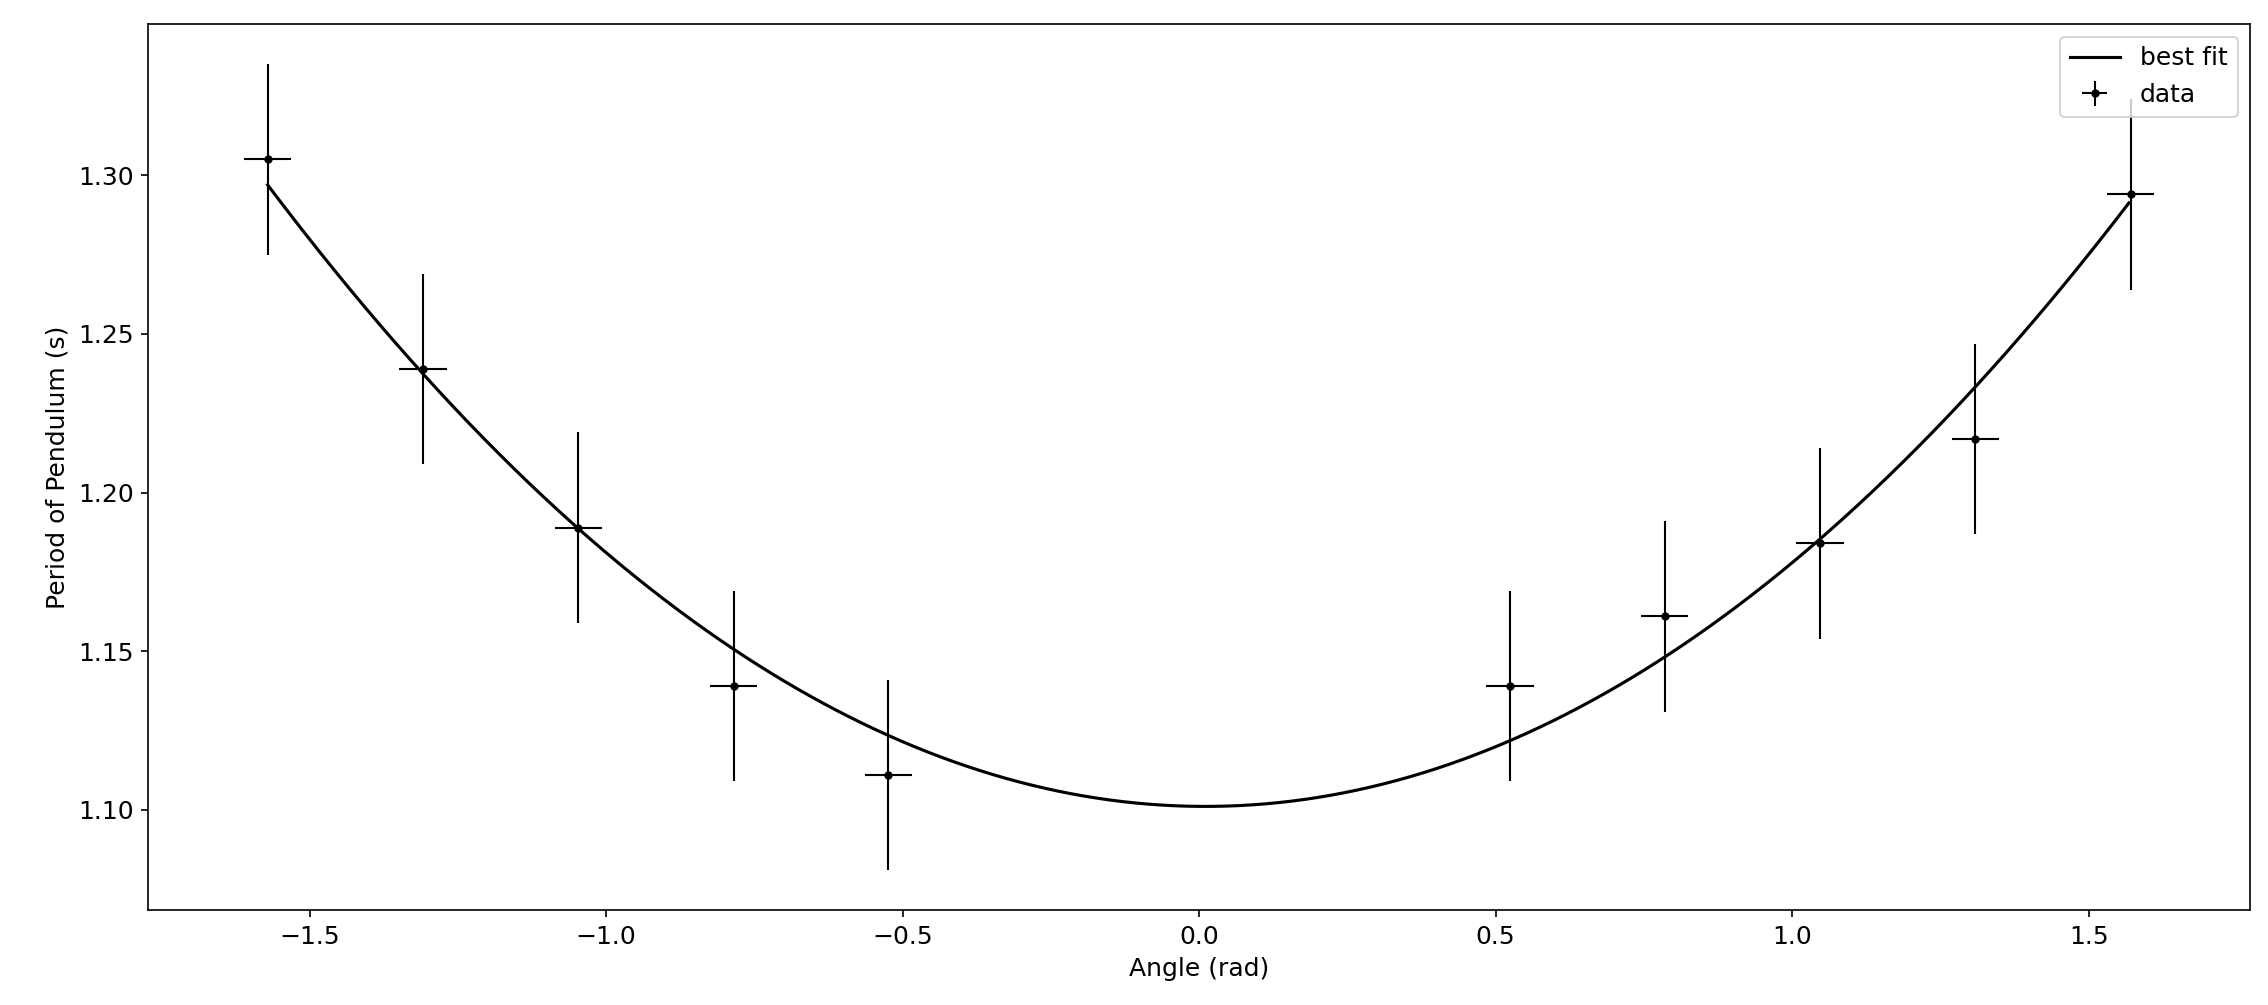
\includegraphics[scale=0.28]{fig_angle.png}
	\caption{\textit{Period of Pendulum (s) vs. Angle (rad)}}
	\center \textit{Note that the horizontal error bar has a length of $\pm$ 0.01 rad, and the vertical error bar has a length of $\pm$ 0.03 second. }

	\label{fig_angle}
\end{figure}

It is observable from \textbf{Figure 2}, that the maximum period $T$  decreases exponentially as the angle gets closer to 0 rad. However, this decrease occurs within an interval of approximately 0.20, which is a negligible difference, attributable to two systematic errors: One being the reducing friction between string and stand as angle gets smaller, and the other one being the decreasing air resistance during pendulum swings as angle gets smaller. Both of these errors decreases the period of the pendulum as the angle gets smaller.

\subsubsection{Graphing and Analysing Figure 3 and Figure 4}

Upon tracking the decay of pendulum's amplitude starting from 1.31 $\pm$ 0.01 radian, a relationship between the angle of pendulum and time is demonstrated in \textbf{Figure 3}. 

\begin{figure}[h]
\begin{minipage}{.5\textwidth}
	\centering
	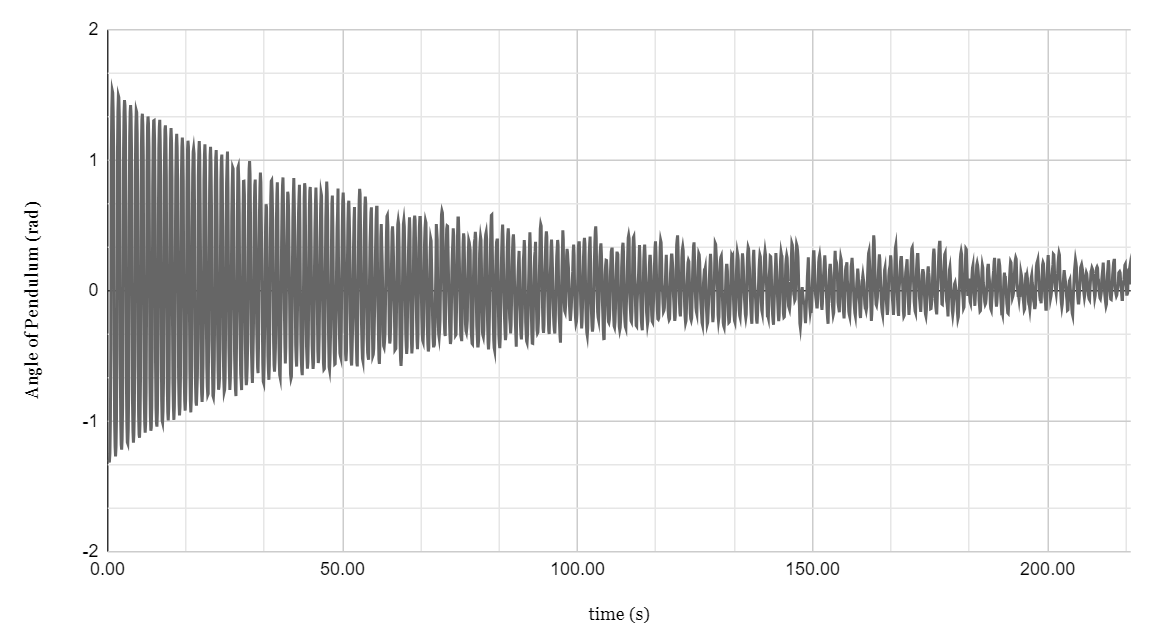
\includegraphics[scale=0.4]{Pendulum_Decay_Chart1.png}
	\caption{\textit{Angle of Pendulum (Rad) vs. Time (s)}}
	\label{fig_angle}
\end{minipage}%
\begin{minipage}{.5\textwidth}
	\centering
	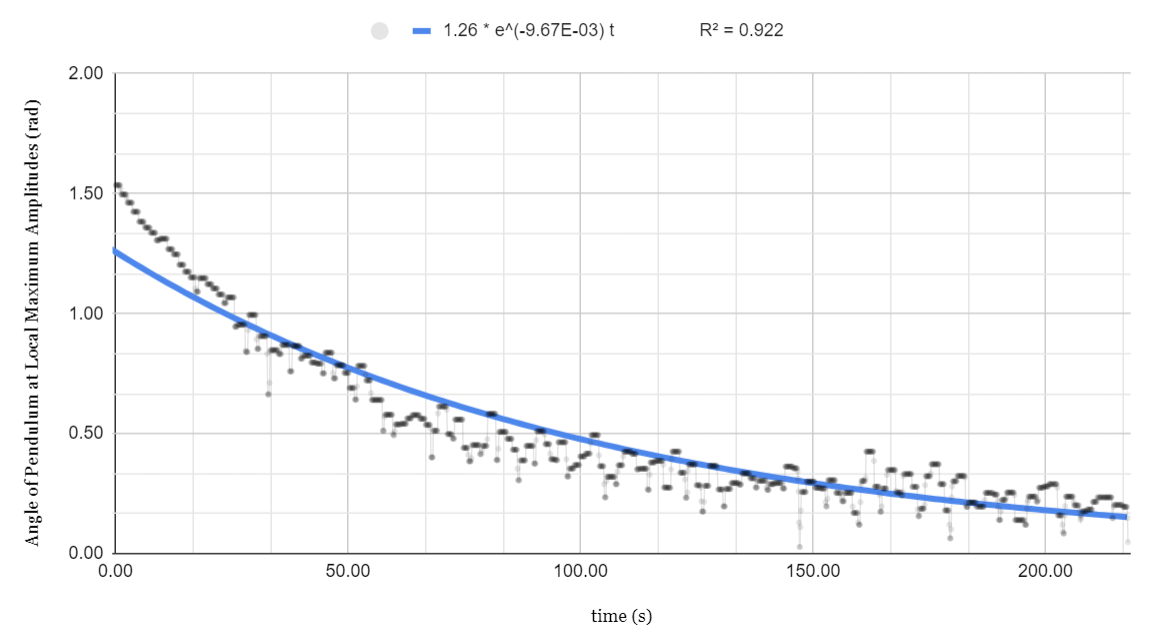
\includegraphics[scale=0.5]{Pendulum_Decay_Chart2.png}
	
	\caption{\textit{Angle of Pendulum at Local Maximum Amplitude (Rad) vs. Time (s)}}
\end{minipage}

	\center \textit{Note that the for both \textbf{Figure 3} and \textbf{Figure 4}, the vertical error bar has a length of $\pm$ 0.01 rad, and the horizontal error bar has a length of $\pm$ 0.03 second. However, these error bars are hardly observable, attributable to large range at both the vertical and horizontal axis, as well as the large number of concentrated data points}
	\label{fig_angle}
\end{figure}

\textbf{Figure 3} is crucial in determining the Q Factor by counting the number of oscillations that occurred in this graph. \\
\indent It is observable from \textbf{Figure 3} that the relationship between the Angle of Pendulum over time is an oscillating cosine function. The maximum amplitude of the pendulum decreases exponentially as time increases. Therefore, taking the angle at all the local maximum amplitude over the entire time interval, along with their respective time, we can construct a new graph of the angle at local maximum amplitude over time in \textbf{Figure 4}. \textbf{Figure 4} is crucial in determining the factor $\tau$, which is used to calculate Q Factor through fitting the function to graph in section 3.3.1.

\subsection{Q Factor Calculation of section 3.2}

\subsubsection{Through Fitting the Function to Graph}

Referencing the gathered data from section 3.2, we can find the release angle of the pendulum:
$$ \theta = 1.31 \pm 0.01rad $$
as well as the maximum period of pendulum:
$$ T = 1.29 \pm 0.03s $$
Substituting in the values to equation , we will fit equation \textbf{(3)} the graph in \textbf{Figure 4}, and find the $\tau$ factor:
\begin{equation}
 \theta = (-1.31 \pm0.01rad) * e^{t/\tau} 
\end{equation}

$$ \therefore \tau \simeq 77.58 \pm 0.03s $$
Further, we calculate Q factor through equation \textbf{(2)}:
$$ \therefore Q=\pi \frac{\tau}{T}=\pi \frac{77.58s \pm 0.03s}{1.29s \pm 0.03s} \simeq 200 \pm 1$$

\noindent Therefore, the Q Factor for the pendulum is 200 $\pm$ 1,
\subsubsection{Through Counting Oscillations}

Through counting oscillation until the 4 \% of the original angle 1.31 $\pm$ 0.01:

\[ \theta_0 * 4 \% = 1.31 rad * 4 \% = 0.05 \pm 0.01 rad \]

\noindent I was able to count 196 $\pm$ 5 oscillations, therefore, the Q factor from counting oscillations is 196 $\pm$ 5. Uncertainty is $\pm$ 5 due to human error on determining the exact point where angle equals 0.05$\pm$0.01rad

\subsubsection{Comparing Q Factor from both methods}

The Q Factor through counting oscillation is very close with the Q Factor through Estimating Periods, with a difference of only $\Delta = 200-196=4$. This difference is covered within the uncertainty from both Q Factor calculations, as $\pm 5 + \pm 1 = \pm 6 \geqslant \Delta $


\subsection{Relationship between Period vs. Length of Pendulum}
\subsubsection{Graphing and Analysing Figure 5}
Through releasing the pendulum from 1.05 $\pm$ 0.01 rad, separately at a length of  30.0 $\pm$ 0.1cm,  25.0 $\pm$ 0.1cm, 20.0 $\pm$ 0.1cm, 15.0 $\pm$ 0.1cm, and 10.0 $\pm$ 0.1cm  from both side of the wooden stand; and recording the period inside the tracker application [1], we were able to gather data and graph the relationship between the period and the corresponding length of the pendulum in \textbf{Figure 5}, as well as the modified log-log graph in \textbf{Figure 6}:

\begin{figure}[!htp]
	\begin{minipage}{.5\textwidth}
	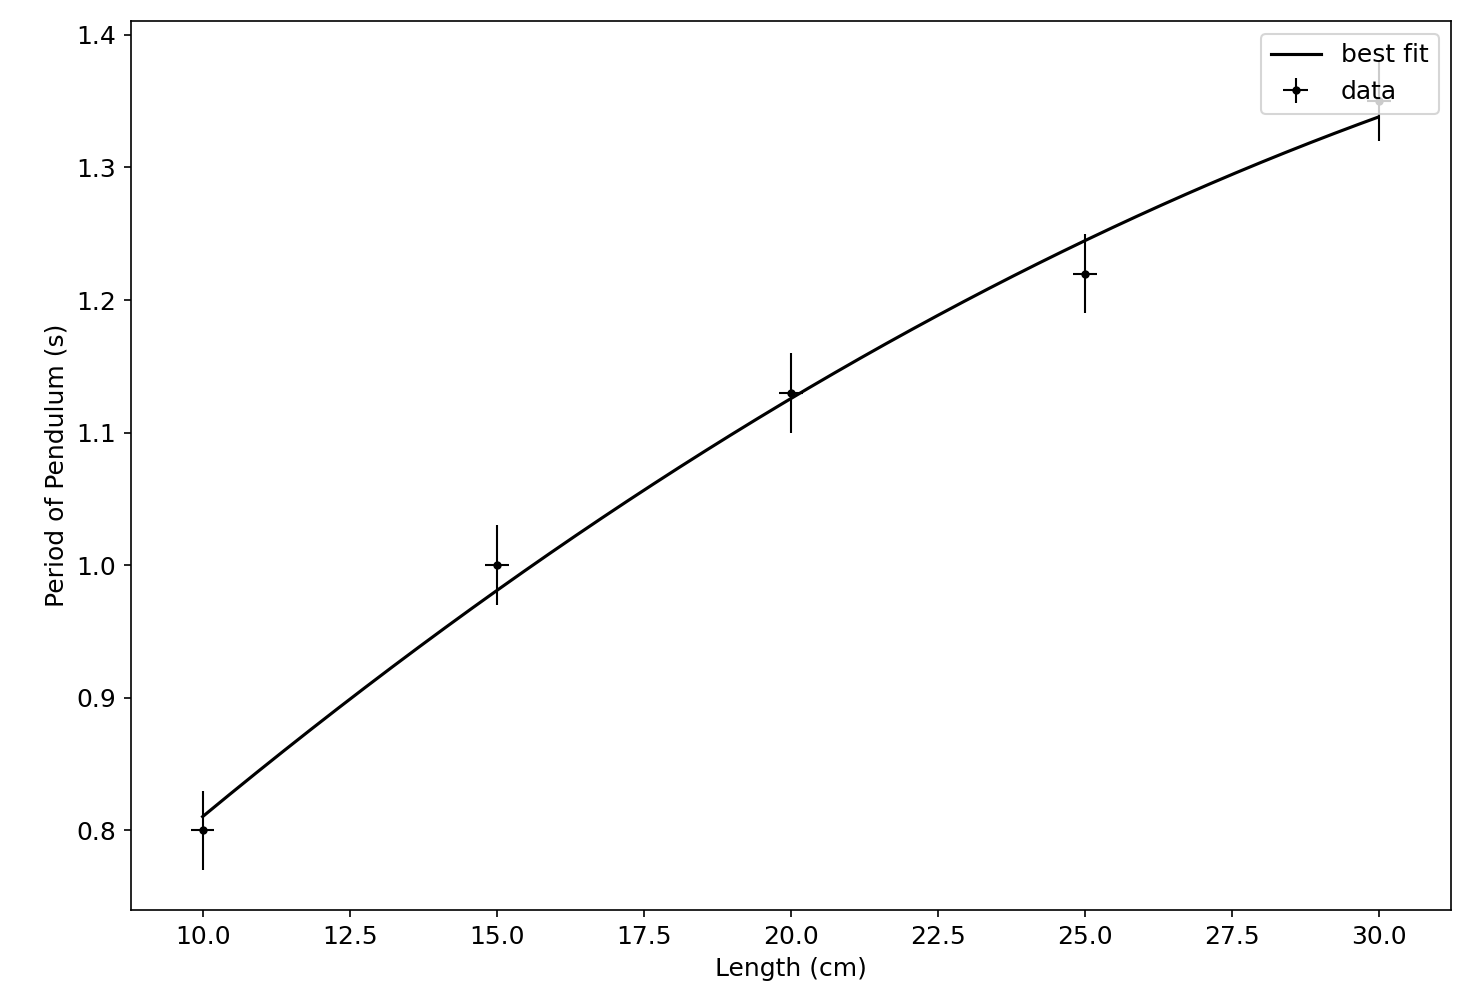
\includegraphics[scale = 0.3]{Pendulum_Length_Image.png}
	\caption{\textit{Period of Pendulum (s) vs. Length (cm)}}
	
	\label{length}
	\end{minipage}%
	\begin{minipage}{.7\textwidth}
		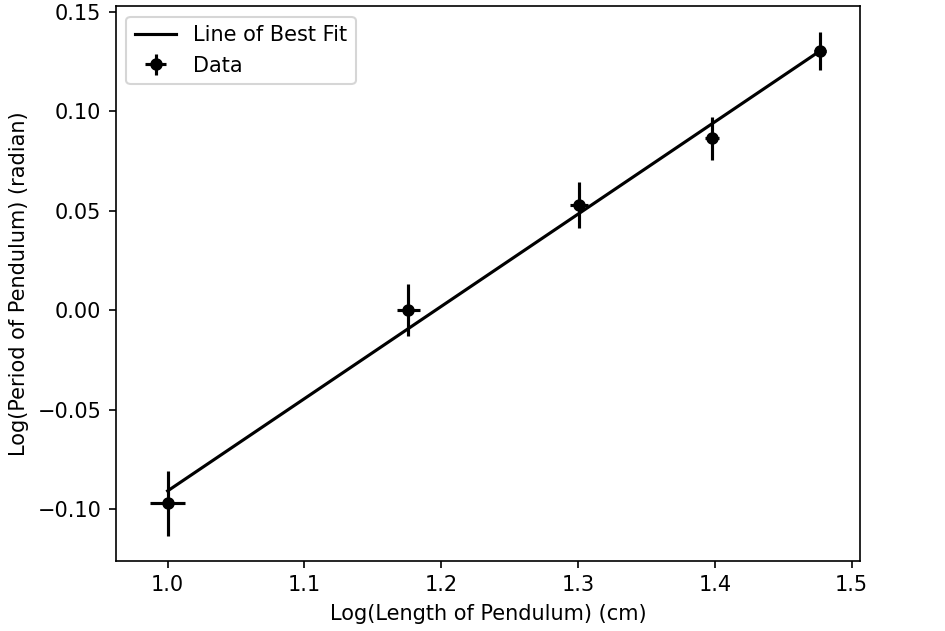
\includegraphics[scale = 0.45]{loglog.png}
	\caption{\textit{log(Period of Pendulum)(s) vs. log(Length)(cm)}}
	\end{minipage}
	\center \textit{Note that for \textbf{Figure 5}, the horizontal error bar has a length of $\pm$ 0.1 cm, and the vertical error bar has a length of $\pm$ 0.03 second. For \textbf{Figure 6}, the horizontal error bar has a length of $\pm$ 0.01 log(cm), and the vertical error bar has a length of $\pm$ 0.007 log(second).}
\end{figure}
It is therefore observable that the maximum period $T$ of pendulum increases logarithmically as length of pendulum increases.
\subsubsection{Calculating and graphing Q Factor vs. Length}
For each of the different length of pendulum, we will calculate the Q Factor through fitting the provided equation \textbf{(3)} - with values of angle and time found in section 3.4.1 - to the graph of Periods vs. Angles until the tenth cycle. We are using the fitting to graph method, as this method will produce results of Q factor with lower uncertainty ($\pm$1, as shown in section 3.3.1) than that from counting oscillations ($\pm$5, as shown in section 3.3.2) Note that since both Period (T) and Time (t) has an uncertainty of $\pm$0.03 seconds, the uncertainty of $\tau$ should be $\pm$ 0.03, and therefore the uncertainty of Q Factor should be $\pm$ 1. This calculation has been demonstrated in section 3.3.1 \\
\indent Using the calculated data of Q Factors, we are able to graph a relationship between the Q Factor and the length of the pendulum in \textbf{Figure 7}. It is therefore observable from \textbf{Figure 7} that Q Factor increases exponentially as length of pendulum increases.

\begin{figure}[!htb]
	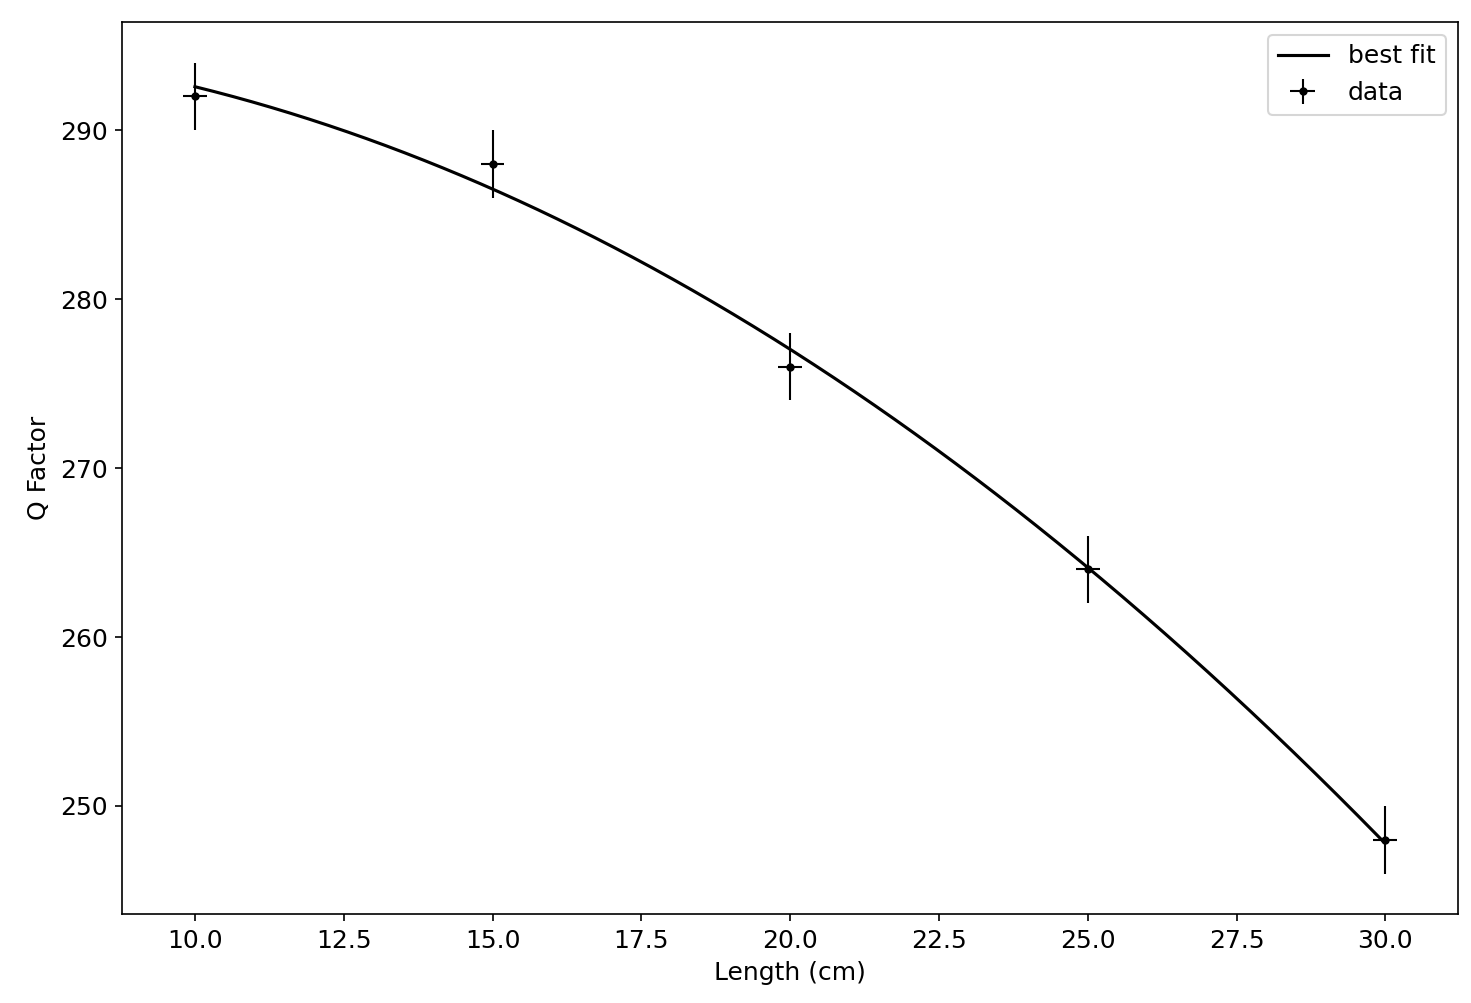
\includegraphics[scale=0.3]{Q_Factor_Length.png}
	\caption{\textit{Q Factor vs. Length (cm)}}
	\center 
	\textit{Note that the horizontal error bar has a length of $\pm$ 0.1 cm, and the vertical error bar has a length of $\pm$ 1. }
	\label{length}
	
\end{figure}

\section{Conclusion}
In this lab report:
\begin{enumerate}
\item Through releasing the pendulum at 1.57 $\pm$ 0.01rad, we plotted the period (with $\pm$ 0.03second uncertainty)against angle in \textbf{Figure 2}, thereby demonstrating that the Maximum Period of pendulum is dependent of the angle. However, this decrease occurs within an interval of approx. 0.20, a negligible decrease of period over the decrease of angle, as caused by two specified error in section 3.2.1.
\item Upon tracking from an angle of 1.31 $\pm$ 0.01rad, we plotted the period (with $\pm$ 0.03second uncertainty) against angle in \textbf{Figure 3}, thereby demonstrating that the amplitude decay exponentially as time increases. Upon calculation in section 3.3, the two Q Factors measurements through different methods, 200 $\pm$ 1 and 196 $\pm$ 5, does agree with each other.
 \end{enumerate}
 
  As both Q Factors agree with each other, we conclude that, within an uncertainty of $\pm$ 1, our calculation does agree with the mathematics model equation \textbf{(1)} given. 
  
\begin{enumerate}
  \item Through releasing the pendulum at 1.05 $\pm$ 0.01rad, and at length 10.0,15.0,20.0,25.0,30.0 $\pm$ 0.1cm, we plotted the period (with $\pm$ 0.03second uncertainty)against angle in \textbf{Figure 5 and 6}, thereby demonstrating that the Maximum Period of pendulum is dependent on its length. As length of pendulum increases, the period of pendulum increases exponentially.
  \item By calculating and graphing 5 Q Factors (292,288,276,264,248 $\pm$ 1) against length (10.0,15.0,20.0,25.0,30.0 $\pm$ 0.1cm) in \textbf{Figure 7}, we demonstrated that the Q Factor of pendulum is dependent on its length. As the length of pendulum increases, the Q Factor of pendulum decreases exponentially. 
 \end{enumerate}
 As a higher Q Factor indicates a lower rate of energy loss and the oscillations die out more slowly [2], this implies that for longer lengths of pendulums, the damping effect will be more significant, as the rate of energy loss will be higher, and the oscillation will die out more quickly. With regards to an uncertainty of $\pm$ 1, this property also agrees with the mathematics model equation \textbf{(1)} given.



\section{Reference List}

[1] Tracker. Tracker Video Analysis and Modeling Tool for Physics Education. (n.d.). https://physlets.org/tracker/ \\

\noindent [2] Lepeshkin, N. (n.d.). Q factor . University of Massachusetts Lowell. \\
https://faculty.uml.edu/pchowdhury/PHYS2690/Supp/Q-factor.pdf 

\end{document}


